\documentclass[11pt,a4paper,oneside]{book}

% ── Essential Typographic & Structural Packages ──
\usepackage[utf8]{inputenc}
\usepackage[T1]{fontenc}
\usepackage{lmodern}
\usepackage[scaled=0.92]{inconsolata} % High-legibility monospaced font
\usepackage[margin=2.2cm,top=2.5cm,bottom=2.5cm,headheight=22pt]{geometry}
\usepackage{microtype}
\usepackage{xcolor}
\usepackage{graphicx}
\usepackage{amsmath,amssymb}
\usepackage{tabularx}
\usepackage{booktabs}
\usepackage{array}
\usepackage{enumitem}
\usepackage{titlesec}
\usepackage{fancyhdr}
\usepackage[most]{tcolorbox}
\usepackage{tikz}
\usetikzlibrary{shapes,arrows,positioning,calc}
\usepackage{float}

% ── HGG Official Corporate Color Palette ──
\definecolor{HGGNavy}{RGB}{6, 23, 57}         % #061739 - Deep Sovereign Navy
\definecolor{HGGBlue}{RGB}{10, 36, 87}        % #0A2457 - Primary Navy
\definecolor{HGGAccentBlue}{RGB}{20, 88, 139} % #14588B - Strategic Blue
\definecolor{HGGCyan}{RGB}{87, 163, 192}      % #57A3C0 - Ice Blue
\definecolor{HGGGold}{RGB}{196, 152, 56}      % #C49838 - Deep Antique Gold
\definecolor{HGGGoldLight}{RGB}{223, 183, 88} % #DFB758 - Bright Accent Gold
\definecolor{HGGCanvas}{RGB}{248, 250, 252}   % #F8FAFC - Off-White Canvas
\definecolor{HGGDarkText}{RGB}{15, 23, 42}    % #0F172A - Executive Slate Text
\definecolor{HGGMutedText}{RGB}{100, 116, 139}% #64748B - Muted Metadata Text
\definecolor{HGGBorder}{RGB}{226, 232, 240}   % #E2E8F0 - Architectural Border
\definecolor{HGGGreen}{RGB}{16, 185, 129}     % #10B981 - Success Green
\definecolor{HGGRed}{RGB}{225, 29, 72}        % #E11D48 - Alert Red
\definecolor{HGGSlate}{RGB}{203, 213, 225}

% ── Hyperref Setup ──
\usepackage{hyperref}
\hypersetup{
    colorlinks=true,
    linkcolor=HGGAccentBlue,
    filecolor=HGGGold,
    urlcolor=HGGAccentBlue,
    citecolor=HGGGold,
    pdftitle={HGG Sanity Studio CMS Administrator and User Operations Manual},
    pdfauthor={THE HINTER GROUP GHANA LTD Development Team},
    pdfsubject={Comprehensive CMS Manual: Create, Update, Delete, Unpublish, and Governance Operations},
    pdfkeywords={HGG, Sanity CMS, Content Studio, Admin Guide, Employee Verification, QR Generator, Ghana},
    pdfpagemode=UseOutlines,
    bookmarksopen=true
}

% ── Chapter & Section Styling (Book Format) ──
\titleformat{\chapter}[display]
  {\filright\bfseries\color{HGGNavy}}
  {\filright\footnotesize\bfseries\color{HGGGold}CHAPTER \thechapter}
  {6pt}
  {\LARGE\bfseries}[\vspace{4pt}{\color{HGGGold}\hrule height 1.2pt}]

\titlespacing*{\chapter}{0pt}{-20pt}{18pt}

\titleformat{\section}
  {\color{HGGNavy}\normalfont\Large\bfseries}
  {\color{HGGGold}\thesection}{1em}{}[\color{HGGBorder}\titlerule]

\titleformat{\subsection}
  {\color{HGGNavy}\normalfont\large\bfseries}
  {\color{HGGAccentBlue}\thesubsection}{0.8em}{}

\titleformat{\subsubsection}
  {\color{HGGAccentBlue}\normalfont\normalsize\bfseries}
  {\thesubsubsection}{0.6em}{}

% ── Header & Footer Setup ──
\pagestyle{fancy}
\fancyhf{}
\renewcommand{\headrulewidth}{0.6pt}
\renewcommand{\headrule}{\hbox to\headwidth{\color{HGGGold}\leaders\hrule height \headrulewidth\hfill}}
\fancyhead[L]{\small\textbf{\color{HGGNavy}THE HINTER GROUP GHANA LTD} \textcolor{HGGMutedText}{|} \footnotesize\color{HGGMutedText}Admin CMS Operations Manual}
\fancyhead[R]{\small\color{HGGGold}\textbf{CONFIDENTIAL}}
\fancyfoot[L]{\footnotesize\color{HGGMutedText}Sanity Studio CMS Administration}
\fancyfoot[C]{\footnotesize\color{HGGMutedText}Accra, Ghana $\cdot$ West Africa}
\fancyfoot[R]{\small\textbf{\color{HGGNavy}\thepage}}

\fancypagestyle{plain}{
  \fancyhf{}
  \renewcommand{\headrulewidth}{0pt}
  \fancyfoot[L]{\footnotesize\color{HGGMutedText}THE HINTER GROUP GHANA LTD — Confidential}
  \fancyfoot[R]{\small\textbf{\color{HGGNavy}\thepage}}
}

% ── Interactive Callout Boxes ──
\newtcolorbox{goldbox}[1][]{
    colback=HGGGold!7,
    colframe=HGGGold,
    coltitle=HGGNavy,
    fonttitle=\bfseries\normalsize,
    title={#1},
    sharp corners,
    rounded corners=southeast,
    arc=3.5mm,
    boxrule=1.2pt,
    left=4.5mm,right=4.5mm,top=3mm,bottom=3mm,
    before skip=9pt,after skip=9pt,
    breakable
}

\newtcolorbox{navybox}[1][]{
    colback=HGGNavy!5,
    colframe=HGGNavy,
    coltitle=white,
    fonttitle=\bfseries\normalsize,
    title={#1},
    sharp corners,
    rounded corners=southeast,
    arc=3.5mm,
    boxrule=1.2pt,
    left=4.5mm,right=4.5mm,top=3mm,bottom=3mm,
    before skip=9pt,after skip=9pt,
    breakable
}

\newtcolorbox{alertbox}[1][]{
    colback=HGGRed!6,
    colframe=HGGRed,
    coltitle=white,
    fonttitle=\bfseries\normalsize,
    title={#1},
    sharp corners,
    rounded corners=southeast,
    arc=3.5mm,
    boxrule=1.2pt,
    left=4.5mm,right=4.5mm,top=3mm,bottom=3mm,
    before skip=9pt,after skip=9pt,
    breakable
}

\newtcolorbox{tipbox}[1][]{
    colback=HGGCyan!8,
    colframe=HGGAccentBlue,
    coltitle=HGGNavy,
    fonttitle=\bfseries\normalsize,
    title={#1},
    sharp corners,
    rounded corners=southeast,
    arc=3mm,
    boxrule=1pt,
    left=4.5mm,right=4.5mm,top=3mm,bottom=3mm,
    before skip=8pt,after skip=8pt,
    breakable
}

% ── List Formatting ──
\setlist[itemize]{leftmargin=*,itemsep=2.5pt,topsep=2.5pt}
\setlist[enumerate]{leftmargin=*,itemsep=2.5pt,topsep=2.5pt}

\begin{document}

% ═════════════════════════════════════════════════════════════════
% COVER PAGE
% ═════════════════════════════════════════════════════════════════
\begin{titlepage}
\pagecolor{HGGNavy}
\color{white}
\vspace*{0.5cm}

\begin{center}
    % Decorative Gold Accent Line
    
\begin{tikzpicture}
        \draw[HGGGoldLight, line width=2.2pt] (0,0) -- (12,0);
        \fill[HGGGoldLight] (6,0) circle (3.2pt);
    \end{tikzpicture}
    \vspace{0.6cm}

    % Official HGG Corporate Logo Container
    \begin{tcolorbox}[
        colback=white,
        colframe=HGGGoldLight,
        boxrule=1.6pt,
        arc=4mm,
        width=3.4cm,
        height=3.4cm,
        valign=center,
        halign=center,
        top=2mm,bottom=2mm,left=2mm,right=2mm
    ]
        \centering
        
\includegraphics[width=2.8cm,height=2.8cm,keepaspectratio]{./Development/frontend/public/assets/logos/Logo/Logo_Logo.png}
    \end{tcolorbox}
    \vspace{0.4cm}

    {\huge \textbf{THE HINTER GROUP GHANA LTD}}\\[0.25cm]
    {\normalsize \textbf{\color{HGGCyan}CONSULTING + VENTURES \textbar\ BROKERAGE}}\\[0.15cm]
    {\footnotesize \color{HGGGoldLight}\textit{Committed to Excellence $\cdot$ Accra, Ghana $\cdot$ West Africa}}\\[0.9cm]

    % Main Document Title Card
    \begin{tcolorbox}[
        colback=HGGBlue!95,
        colframe=HGGGold,
        boxrule=1.5pt,
        arc=4mm,
        width=0.96\textwidth,
        halign=center,
        top=6mm,bottom=6mm
    ]
        {\LARGE \textbf{\color{white}SANITY STUDIO CMS}}\\[0.2cm]
        {\LARGE \textbf{\color{HGGGoldLight}ADMINISTRATOR \& USER OPERATIONS MANUAL}}\\[0.35cm]
        {\color{HGGSlate}\rule{0.6\textwidth}{0.5pt}}\\[0.35cm]
        {\normalsize \color{HGGCanvas}Authoritative Operating Guide for Content Governance, Dynamic Publishing,}\\[0.1cm]
        {\normalsize \color{HGGCanvas}Personnel Identity Verification, Employee QR Generation, and Data Management}
    \end{tcolorbox}

    \vfill

    % Metadata Registry Card
    \begin{tcolorbox}[
        colback=white,
        colframe=HGGGoldLight,
        boxrule=1.2pt,
        arc=3mm,
        width=0.96\textwidth,
        left=6mm,right=6mm,top=4mm,bottom=4mm
    ]
    \small\color{HGGDarkText}
    \begin{tabularx}{\textwidth}{@{}lX@{}}
        \textbf{\color{HGGNavy}Target Audience:} & Executive Leadership, Communications Desk \& CMS Administrators \\
        \addlinespace[2pt]
        \textbf{\color{HGGNavy}Production Portal:} & \url{https://hintergroupghana.com/studio} \\
        \addlinespace[2pt]
        \textbf{\color{HGGNavy}Live Website URL:} & \url{https://hintergroupghana.com} \\
        \addlinespace[2pt]
        \textbf{\color{HGGNavy}Authentication:} & Federated GitHub OAuth via Google SSO (\texttt{hintergroup.dev@gmail.com}) \\
        \addlinespace[2pt]
        \textbf{\color{HGGNavy}Platform Stack:} & Sanity.io Studio v3 Headless CMS $\cdot$ Next.js 16 Edge Rendering \\
        \addlinespace[2pt]
        \textbf{\color{HGGNavy}Document Classification:} & \textbf{\color{HGGRed}CONFIDENTIAL — INTERNAL USE ONLY} \\
        \addlinespace[2pt]
        \textbf{\color{HGGNavy}Publication Date:} & September 2026 \\
    \end{tabularx}
    \end{tcolorbox}

    \vspace{0.4cm}
    
\begin{tikzpicture}
        \draw[HGGGoldLight, line width=2.2pt] (0,0) -- (12,0);
        \fill[HGGGoldLight] (6,0) circle (3.2pt);
    \end{tikzpicture}
\end{center}
\end{titlepage}

\nopagecolor
\color{HGGDarkText}
\frontmatter

% ═════════════════════════════════════════════════════════════════
% ABSTRACT & SCOPE
% ═════════════════════════════════════════════════════════════════
\chapter*{Notice of Confidentiality \& Executive Scope}
\addcontentsline{toc}{chapter}{Notice of Confidentiality \& Executive Scope}

\begin{navybox}[Confidential Institutional Governance Notice]
This document contains proprietary operational instructions and security protocols governing the official digital content management infrastructure of \textbf{THE HINTER GROUP GHANA LTD (HGG)}. Access to this manual and the embedded administrative Content Studio is restricted to authorized executive officers, corporate communications personnel, and designated system administrators. Unauthorized distribution, disclosure, or reproduction in whole or in part is strictly prohibited.
\end{navybox}

\vspace{0.4cm}

\section*{Executive Abstract}
This manual provides a thorough, step-by-step operational handbook for managing all dynamic content across the official corporate web platform of \textbf{THE HINTER GROUP GHANA LTD} (\url{https://hintergroupghana.com}) using the embedded \textbf{Sanity Studio CMS} portal (\url{https://hintergroupghana.com/studio}).

Engineered as a modern headless Content Operating System, Sanity Studio empowers HGG leadership and communications personnel to create, edit, unpublish, and permanently remove corporate data in real-time with zero programming knowledge. The manual delivers comprehensive instructions for executing full lifecycle data operations (\textbf{Create}, \textbf{Update}, \textbf{Delete}, \textbf{Unpublish}, and \textbf{Restore}) across all nine institutional content desks:
\begin{itemize}[leftmargin=1.2cm]
  \item \textbf{Global Site Settings:} Centralized management of corporate identity, headquarters address, phone, contact emails, and social endpoints.
  \item \textbf{Leadership \& Governance:} Executive member profiles, official designations, high-resolution portraits, and biographical modals.
  \item \textbf{Employee ID \& Personnel Verification:} Registration of verified employees, security badges, and clearance tiers.
  \item \textbf{Employee QR ID Card Generator:} Studio tool generating print-ready cryptographic QR codes and live physical badge previews.
  \item \textbf{Core Service Pillars \& 9 Priority Sectors:} Real-time customization of capabilities, deliverables, and industry corridors.
  \item \textbf{Projects \& Strategic Initiatives:} Deal milestone trackers, structured deliverables, and confidentiality shielding controls.
  \item \textbf{Insights \& Newsroom Hub:} Dynamic thought leadership article authoring, rich text formatting, and category filtering.
  \item \textbf{Legal Compliance Pages:} Dynamic governance of Privacy Policy and Terms of Service documents.
\end{itemize}

\clearpage

% ═════════════════════════════════════════════════════════════════
% TABLE OF CONTENTS
% ═════════════════════════════════════════════════════════════════
\tableofcontents
\clearpage

\mainmatter

% ─────────────────────────────────────────────────────────────────
% CHAPTER 1
% ─────────────────────────────────────────────────────────────────
\chapter{Sanity Studio Architecture \& Strategic Overview}
\label{chap:architecture}

\section{What is Sanity Studio?}
Sanity Studio is an enterprise-grade, open-source Content Management System (CMS) built on top of Sanity's real-time Content Lake. Rather than using an external dashboard, HGG's Content Studio is embedded natively directly within your corporate web application:
\begin{center}
  \Large\bfseries\url{https://hintergroupghana.com/studio}
\end{center}

\begin{figure}[H]
\centering
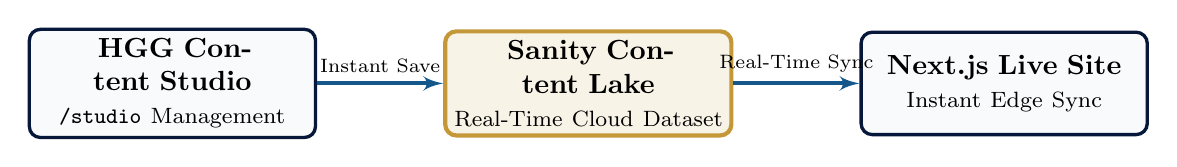
\begin{tikzpicture}[node distance=1.8cm, auto]
  \tikzstyle{block} = [rectangle, draw=HGGNavy, fill=HGGCanvas, text width=3.4cm, text centered, rounded corners, minimum height=1.3cm, line width=1.2pt]
  \tikzstyle{cloud} = [rectangle, draw=HGGGold, fill=HGGGold!12, text width=3.4cm, text centered, rounded corners, minimum height=1.3cm, line width=1.5pt]
  \tikzstyle{line} = [draw=HGGAccentBlue, -latex', line width=1.5pt]

  \node [block] (editor) {\textbf{HGG Content Studio}\\\footnotesize\texttt{/studio} Management};
  \node [cloud, right=1.6cm of editor] (lake) {\textbf{Sanity Content Lake}\\\footnotesize Real-Time Cloud Dataset};
  \node [block, right=1.6cm of lake] (site) {\textbf{Next.js Live Site}\\\footnotesize Instant Edge Sync};

  \path [line] (editor) -- node [above] {\scriptsize Instant Save} (lake);
  \path [line] (lake) -- node [above] {\scriptsize Real-Time Sync} (site);
\end{tikzpicture}
\caption{Real-Time Content Publishing Architecture}
\label{fig:architecture}
\end{figure}

\section{Static vs. Dynamic Content Boundary}
To maintain the highest levels of corporate security, brand integrity, and regulatory compliance, the HGG web platform enforces a strict boundary between immutable code frameworks and editable CMS modules:

\begin{table}[H]
\centering
\small
\begin{tabularx}{\textwidth}{lXX}
  \toprule
  \textbf{Content Classification} & \textbf{Examples \& Placement} & \textbf{Governance Model} \\
  \midrule
  \textbf{Static Brand Framework} & Company Mission, Vision, 8 Core Values, 6-Stage Strategic Approach, Governance Tenets. & Hardcoded into Next.js application codebase for immutable institutional integrity. \\
  \addlinespace[3pt]
  \textbf{Dynamic CMS Modules} & Executive Biographies, Employee Credentials, QR ID Cards, Priority Sectors, Projects, Insights Articles, Contact Endpoints, Legal Policies. & 100\% manageable in real time via Sanity Studio without developer intervention. \\
  \bottomrule
\end{tabularx}
\caption{Classification of Website Data Architecture}
\label{tab:content_boundary}
\end{table}

\section{Core Operational Capabilities Handed Over}
With Sanity Studio, HGG possesses complete administrative sovereignty over its public communications:
\begin{enumerate}
  \item \textbf{Instant Global Updates:} Content updates published in the Studio appear on the public website within seconds without rebuilding or redeploying the site.
  \item \textbf{Real-Time Collaborative Drafting:} Every stroke of text is preserved instantly in private draft state, preventing accidental data loss during network disruptions.
  \item \textbf{Granular Revision Timeline:} Every change made by any editor is logged with timestamps, allowing administrators to review changes and restore prior versions at will.
  \item \textbf{Personnel Verification Authority:} The HGG administrative team can independently issue, modify, suspend, or revoke cryptographic Employee ID credentials and print physical QR cards.
\end{enumerate}

% ─────────────────────────────────────────────────────────────────
% CHAPTER 2
% ─────────────────────────────────────────────────────────────────
\chapter{Authentication, Sign-In Protocol \& User Roles}
\label{chap:auth}

\section{Accessing the Live Portal}
Administrators and editors can access the Studio from any modern web browser on desktop, tablet, or mobile devices by visiting:
\begin{center}
  \Large\bfseries\url{https://hintergroupghana.com/studio}
\end{center}

\begin{goldbox}[Authentication Architecture: Federated Google SSO via GitHub]
\textbf{Crucial Credential Clarification:}
\begin{itemize}
  \item The credentials \textbf{\texttt{hintergroupdev}} and \textbf{\texttt{hintergroup1234}} are \textbf{not} standalone native GitHub username/password credentials.
  \item When opening the Studio login screen, always click \textbf{``Sign in with GitHub''}.
  \item If an active GitHub session already exists in your browser, Sanity Studio opens immediately.
  \item If prompted by GitHub, click \textbf{``Sign in with Google''} and select \textbf{\texttt{hintergroup.dev@gmail.com}} with Google password \textbf{\texttt{hintergroup1234}}.
\end{itemize}
\end{goldbox}

\section{Step-by-Step Sign-In Sequence}
\begin{enumerate}[leftmargin=*,label=\textbf{Step \arabic*:}]
  \item Open your web browser and navigate to \url{https://hintergroupghana.com/studio}.
  \item Click the \textbf{Sign in with GitHub} button.
  \item If GitHub is already signed in on your computer, Sanity Studio will immediately authenticate and load the HGG Content Management workspace.
  \item If GitHub prompts for authentication:
    \begin{itemize}[leftmargin=1.2cm]
      \item Click \textbf{Sign in with Google} (or \textit{Continue with Google}).
      \item Choose the account: \textbf{\texttt{hintergroup.dev@gmail.com}}.
      \item Enter the Google password: \textbf{\texttt{hintergroup1234}}.
      \item Authorize Sanity Studio to access your GitHub profile.
    \end{itemize}
  \item You will enter the Studio with full administrative ownership.
\end{enumerate}

\section{Inviting Team Members \& Assigning Editorial Roles}
To delegate day-to-day writing or HR verification tasks to colleagues without sharing master account credentials, administrators can invite team members using their individual corporate email addresses:

\begin{enumerate}[leftmargin=*,label=\textbf{Step \arabic*:}]
  \item Navigate to the official Sanity Management Console:
    \begin{center}
      \url{https://www.sanity.io/manage}
    \end{center}
  \item Sign in using GitHub / Google (\texttt{hintergroup.dev@gmail.com}).
  \item Select project \textbf{HGG} (Project ID: \texttt{0rqjd271}).
  \item Click the \textbf{Members} tab in the top navigation bar.
  \item Click the green \textbf{Invite Member} button.
  \item Enter the colleague's email address and assign an appropriate role:
    \begin{itemize}[leftmargin=1.2cm]
      \item \textbf{Administrator:} Unrestricted access across all datasets, schemas, user permissions, and billing settings.
      \item \textbf{Editor:} Full operational rights to create, edit, publish, and delete articles, employee records, projects, and site settings, but cannot delete the project or alter billing.
    \end{itemize}
  \item Click \textbf{Send Invite}. The recipient will receive an activation email from Sanity and can subsequently log in directly at \url{https://hintergroupghana.com/studio}.
\end{enumerate}

% ─────────────────────────────────────────────────────────────────
% CHAPTER 3
% ─────────────────────────────────────────────────────────────────
\chapter{Studio Interface Layout \& Navigation Panes}
\label{chap:interface}

\section{Three-Pane Architectural Layout}
Sanity Studio employs an intuitive three-pane progressive navigation structure:

\begin{figure}[H]
\centering
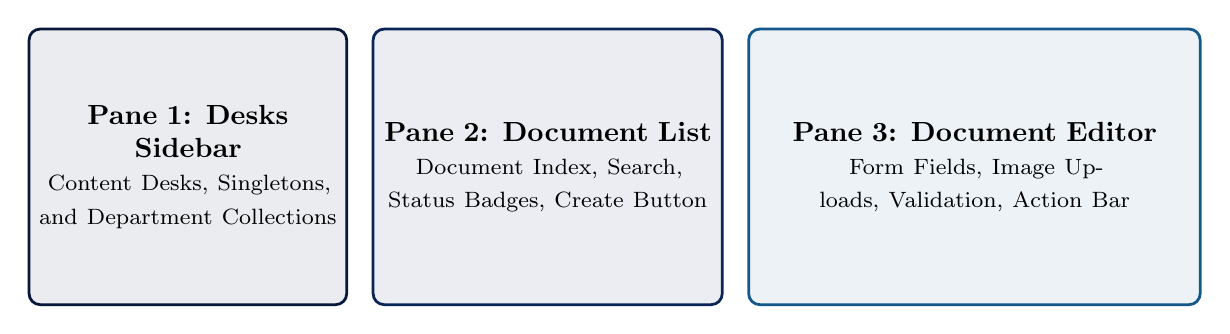
\begin{tikzpicture}[node distance=0.5cm, auto]
  \tikzstyle{pane1} = [rectangle, draw=HGGNavy, fill=HGGNavy!8, text width=3.8cm, text centered, rounded corners, minimum height=3.5cm, line width=1pt]
  \tikzstyle{pane2} = [rectangle, draw=HGGBlue, fill=HGGBlue!8, text width=4.2cm, text centered, rounded corners, minimum height=3.5cm, line width=1pt]
  \tikzstyle{pane3} = [rectangle, draw=HGGAccentBlue, fill=HGGAccentBlue!8, text width=5.5cm, text centered, rounded corners, minimum height=3.5cm, line width=1pt]

  \node [pane1] (p1) {\textbf{Pane 1: Desks Sidebar}\\\footnotesize Content Desks, Singletons, and Department Collections};
  \node [pane2, right=0.3cm of p1] (p2) {\textbf{Pane 2: Document List}\\\footnotesize Document Index, Search, Status Badges, Create Button};
  \node [pane3, right=0.3cm of p2] (p3) {\textbf{Pane 3: Document Editor}\\\footnotesize Form Fields, Image Uploads, Validation, Action Bar};
\end{tikzpicture}
\caption{Sanity Studio Three-Pane Workspace Organization}
\label{fig:panes}
\end{figure}

\section{Top Navigation Header}
The horizontal bar across the very top of the Studio contains:
\begin{itemize}
  \item \textbf{Tool Switcher:} Allows switching between \textbf{Content} (the primary CMS document editor) and \textbf{Employee QR ID Card Generator} (the dedicated card generation and printing tool).
  \item \textbf{Global Search Bar:} Allows instant searching across all documents, titles, author names, and employee ID codes in the dataset.
  \item \textbf{User Account Menu:} Displays the currently logged-in user profile, theme controls, and logout button.
\end{itemize}

\section{The Document Editor Pane}
When a document is opened in Pane 3, you will find:
\begin{itemize}
  \item \textbf{Breadcrumb Header:} Shows the current desk and document title.
  \item \textbf{Document Timeline (History Icon):} Located in the top right corner. Clicking this icon opens the chronological revision history panel.
  \item \textbf{Field Form Controls:} Text fields, rich text blocks, image dropzones, reference pickers, and toggles.
  \item \textbf{Validation Badges:} Displays green checkmarks when all mandatory fields are valid, or red markers highlighting missing required fields.
  \item \textbf{Bottom Publishing Action Bar:} Houses the live status indicator (\textit{Published}, \textit{Draft}, \textit{Changes not published}), the primary green \textbf{Publish} button, and the Document Actions menu (\texttt{...}).
\end{itemize}

% ─────────────────────────────────────────────────────────────────
% CHAPTER 4
% ─────────────────────────────────────────────────────────────────
\chapter{Core Content Operations: Create, Update, Delete \& Restore}
\label{chap:crud}

\section{Overview of Content Lifecycle}
Every piece of information inside Sanity Studio moves through a structured, safe editorial lifecycle:
\begin{center}
  \textbf{Draft (Auto-Saved)} $\longrightarrow$ \textbf{Validation} $\longrightarrow$ \textbf{Publish (Live)} $\longleftrightarrow$ \textbf{Unpublish / Archive}
\end{center}

\section{Creating New Documents (Step-by-Step)}
Follow this standardized procedure to author new content (e.g., adding an Insights Article, an Executive Profile, or an Employee ID Record):

\begin{enumerate}[leftmargin=*,label=\textbf{Step \arabic*:}]
  \item In Pane 1 (left sidebar), click on the target desk (e.g., \textbf{Insights \& News Articles}).
  \item In Pane 2 (document list), click the \textbf{Create new} button (represented by a \textbf{+} plus icon or ``Create new'' text at the top of the pane).
  \item A blank form will open in Pane 3.
  \item Enter all required fields:
    \begin{itemize}[leftmargin=1.2cm]
      \item Fields marked with a red asterisk (\textcolor{HGGRed}{\textbf{*}}) are mandatory.
      \item For fields with a \textbf{Generate} button next to them (such as URL Slugs), click \textbf{Generate} to automatically derive a web-safe identifier from the title.
    \end{itemize}
  \item \textbf{Draft Auto-Saving:} Notice that as you type, the bottom bar indicates \textbf{``Draft''}. Sanity automatically saves your work every millisecond. You do not need to press ``Save''.
  \item \textbf{Publishing Live:} Once all required fields are filled and valid, click the large green \textbf{Publish} button in the bottom right corner.
  \item The status immediately transitions to a green checkmark: \textbf{``Published''}. The new content is now instantly accessible on the live website.
\end{enumerate}

\section{Updating \& Modifying Existing Documents}
To modify text, replace photos, or update contact information on live pages:

\begin{enumerate}[leftmargin=*,label=\textbf{Step \arabic*:}]
  \item Select the appropriate desk from the sidebar.
  \item Click on the existing document you wish to modify.
  \item Edit the desired fields directly.
  \item Notice the bottom status bar turns into a yellow dot labeled \textbf{``Changes not published''}.
  \item \textit{Important:} Visitors to your live website continue to see the previously published version until you click \textbf{Publish}.
  \item Review your revisions, then click the green \textbf{Publish} button. The live site updates immediately.
\end{enumerate}

\section{Version History, Audit Trails \& Reverting Edits}
Sanity maintains an immutable, chronological ledger of every keystroke and change made to every document:

\begin{enumerate}[leftmargin=*,label=\textbf{Step \arabic*:}]
  \item Open the document in Pane 3.
  \item In the top right corner of the editor pane, click the \textbf{Timeline} (clock/history) icon.
  \item A slide-out panel will display every revision, tagged with the editor's name and exact date/timestamp.
  \item Click on any previous point in time to inspect exactly how the document looked at that moment (additions are highlighted in green, deletions in red).
  \item To undo a mistake and revert to an older state, click \textbf{Restore this version}.
  \item Click \textbf{Publish} to push the restored version back to the live website.
\end{enumerate}

\section{Deleting Documents Permanently}
When an article, test data, or obsolete record must be eradicated completely from the database:

\begin{enumerate}[leftmargin=*,label=\textbf{Step \arabic*:}]
  \item Open the document you wish to delete in Pane 3.
  \item Look at the bottom right corner next to the green Publish button. Click the \textbf{Document Actions} button (represented by an ellipsis \textbf{\texttt{...}} or small dropdown arrow).
  \item In the context menu, select \textbf{Delete}.
  \item A confirmation dialog will appear warning: \textit{``Are you sure you want to delete this document? This action cannot be undone.''}
  \item Click the red \textbf{Delete} button to confirm.
  \item The document is permanently expunged from the database and immediately disappears from the live site.
\end{enumerate}

\section{Unpublishing \& Archiving Content (Recommended Alternative)}
In corporate environments, completely deleting documents is often undesirable because valuable historical text, photography, or employee records are permanently lost. Sanity provides a superior alternative: \textbf{Unpublishing}.

\begin{tipbox}[Best Practice: Unpublish Instead of Delete]
When an initiative concludes, an employee is on leave, or an article is under review, use \textbf{Unpublish}. The document will immediately vanish from the public website, but will remain safely stored as a private draft in your Studio for future reference or re-activation.
\end{tipbox}

\begin{enumerate}[leftmargin=*,label=\textbf{Step \arabic*:}]
  \item Open the live document.
  \item Click the Document Actions menu (\textbf{\texttt{...}}) in the bottom right corner.
  \item Select \textbf{Unpublish}.
  \item The document's status changes from \textit{Published} back to \textit{Draft}.
  \item The document is immediately removed from the live website and XML sitemap, but remains available in your Studio desk list whenever you want to publish it again.
\end{enumerate}

\section{Duplicating Documents as Templates}
To rapidly author a new article or project based on the formatting of an existing one:
\begin{enumerate}
  \item Open the source document.
  \item Click the Document Actions menu (\textbf{\texttt{...}}).
  \item Select \textbf{Duplicate}.
  \item A fresh copy titled \textit{``[Copy of...]''} will be generated in draft state.
  \item Modify the title, slug, and body copy, then click \textbf{Publish}.
\end{enumerate}

% ─────────────────────────────────────────────────────────────────
% CHAPTER 5
% ─────────────────────────────────────────────────────────────────
\chapter{Global Site Settings \& Institutional Branding}
\label{chap:settings}

\section{The Master Singleton Concept}
In Pane 1, the very first item is \textbf{Global Site Settings}. This is a \textbf{Singleton document} (meaning there is exactly one master record in the system). It acts as the central nerve center for all institutional contact and branding information across the entire website.

\section{Configurable Corporate Fields}
\begin{table}[H]
\centering
\small
\begin{tabularx}{\textwidth}{lXl}
  \toprule
  \textbf{Setting Field} & \textbf{Operational Context \& Placement} & \textbf{Format / Example} \\
  \midrule
  \textbf{Company Legal Name} & Appears in Navbar, Footer, and legal metadata. & \texttt{THE HINTER GROUP GHANA LTD} \\
  \textbf{Corporate Tagline} & Sub-heading displayed across browser tabs and SEO. & \texttt{Consulting + Ventures | Brokerage} \\
  \textbf{Contact Email} & Receiving inquiry address in Footer and Contact Desk. & \texttt{info@hintergroupghana.com} \\
  \textbf{Primary Phone} & Clickable corporate phone endpoint in Header/Footer. & \texttt{+233 (0) 30 200 0000} \\
  \textbf{Office Headquarters} & Physical address shown on Contact Page and Footer. & \texttt{The Octagon, Block D, Accra, Ghana} \\
  \textbf{LinkedIn URL} & Official corporate company profile link. & Full HTTPS URL \\
  \textbf{X (Twitter) URL} & Official communications feed link. & Full HTTPS URL \\
  \textbf{Default Social Image} & Fallback $1200\times630$px card used when sharing links. & High-res PNG/JPG upload \\
  \bottomrule
\end{tabularx}
\caption{Global Site Settings Configuration Fields}
\label{tab:site_settings}
\end{table}

\begin{goldbox}[Automatic Site-Wide Propagation]
When an administrator modifies the corporate phone number, email address, or office suite in Global Site Settings and clicks \textbf{Publish}, the update propagates across every page of the website (Navigation Bar, Mobile Drawer, Contact Us, Footer, and SEO Meta) in real time.
\end{goldbox}

% ─────────────────────────────────────────────────────────────────
% CHAPTER 6
% ─────────────────────────────────────────────────────────────────
\chapter{Leadership \& Governance Management}
\label{chap:leadership}

\section{The Leadership Desk Overview}
The \textbf{Leadership \& Governance} desk controls all executive profile cards and biographical modal windows published on the official \url{https://hintergroupghana.com/leadership} page.

\section{Profile Fields Specification}
\begin{itemize}
  \item \textbf{Full Name:} Executive’s legal and professional name including honorary and military titles (\textit{e.g., Charles N. Hammond, Maj. Gen. Matthew Essien --- GAF (Rtd.), Lt. Commander Daniel Kotei --- USN (Rtd.)}).
  \item \textbf{Executive Title / Role:} Corporate governance designation (\textit{e.g., Chairman \& Founder, Strategic Coordination \& Stakeholder Engagement}).
  \item \textbf{Display Priority Order:} An integer number controlling card positioning:
    \begin{itemize}
      \item \texttt{1} = Chairman \& Founder (anchors the top-left spotlight card).
      \item \texttt{2}, \texttt{3}, \texttt{4}, \dots = Sequenced executive committee members.
    \end{itemize}
  \item \textbf{Executive Portrait:} Clean, high-resolution portrait photograph.
  \item \textbf{Short Biography (Front Card):} A concise 2-sentence summary visible directly on the public card face.
  \item \textbf{Comprehensive Institutional Biography (Popup Modal):} The full professional background displayed when website visitors click \textit{``Read Full Biography''}. Supports multi-paragraph rich text formatting.
  \item \textbf{Core Governance Responsibilities:} Bullet points highlighting executive oversight domains (\textit{e.g., Strategic Direction, Consortium Structuring, Institutional Partnerships}).
\end{itemize}

\begin{tipbox}[Portrait Photography Standards]
For executive cards to display with maximum aesthetic appeal:
\begin{itemize}
  \item Use a vertical aspect ratio ($3:4$ or $4:5$).
  \item Minimum resolution: $1200\times1500$ pixels.
  \item Professional corporate attire with clean architectural or solid backgrounds.
\end{itemize}
\end{tipbox}

% ─────────────────────────────────────────────────────────────────
% CHAPTER 7
% ─────────────────────────────────────────────────────────────────
\chapter{Employee ID \& Personnel Verification System}
\label{chap:verification}

\section{Purpose of the Personnel Verification Database}
To protect HGG against fraudulent impersonation and verify executive credentials before international partners, government ministries, and financial institutions, the platform incorporates an authoritative \textbf{Personnel Verification Engine} accessible globally at:
\begin{center}
  \Large\bfseries\url{https://hintergroupghana.com/verify/[id]}
\end{center}

\section{Registering a New Employee or Official}
To issue official verification credentials to a staff member or executive:
\begin{enumerate}[leftmargin=*,label=\textbf{Step \arabic*:}]
  \item In Pane 1, click the \textbf{Employee ID \& Verification} desk.
  \item Click \textbf{Create new} (+).
  \item \textbf{Employee ID Code:} Enter the unique corporate code formatted as \texttt{HGG-XXX} (e.g., \texttt{HGG-001}, \texttt{HGG-002}).
  \item \textbf{Full Legal Name:} Enter the employee's official name.
  \item \textbf{Designation / Role:} Official position held within the firm.
  \item \textbf{Department:} Corporate division (\textit{e.g., Executive Office, Strategic Advisory, Project Operations, Commercial Brokerage}).
  \item \textbf{Clearance Tier:} Select from the dropdown:
    \begin{itemize}
      \item \textbf{Executive Leadership} (Highest institutional authority)
      \item \textbf{Senior Advisory} (Advisory board and senior consultants)
      \item \textbf{Operational Associate} (Full-time operational personnel)
    \end{itemize}
  \item \textbf{Credential Status:}
    \begin{itemize}
      \item \textcolor{HGGGreen}{\textbf{Active}} = Displays green shield badge: \textbf{IDENTITY VERIFIED}.
      \item \textcolor{HGGGold}{\textbf{Suspended}} = Displays yellow warning badge: \textbf{CREDENTIAL SUSPENDED}.
      \item \textcolor{HGGRed}{\textbf{Revoked / Archived}} = Displays red warning: \textbf{CREDENTIAL REVOKED}.
    \end{itemize}
  \item \textbf{Issue Date \& Expiry Date:} Set the credential validity window.
  \item \textbf{Official Portrait:} Upload the employee's corporate ID photograph.
  \item Click the green \textbf{Publish} button. The verification route is immediately live and verifiable worldwide.
\end{enumerate}

\begin{alertbox}[Strict Confidentiality \& Data Protection Policy]
In compliance with the \textit{Ghana Data Protection Act, 2012 (Act 843)}, the public verification page strictly displays \textbf{professional public credentials only}.
\textbf{NEVER} enter personal confidential data (such as Home Residential Address, Date of Birth, Personal Mobile Number, or National ID/Passport Numbers) into the CMS.
\end{alertbox}

% ─────────────────────────────────────────────────────────────────
% CHAPTER 8
% ─────────────────────────────────────────────────────────────────
\chapter{Employee QR ID Card Generator Tool}
\label{chap:qrtool}

\section{Dedicated Studio Generator Tool}
In addition to the standard document desks, Sanity Studio features an integrated custom tool accessible via the top navigation bar:
\begin{center}
  \textbf{Top Header Bar} $\longrightarrow$ Click \textbf{[Employee QR ID Card Generator]}
\end{center}

\section{Operating the QR Card Generator}
\begin{enumerate}[leftmargin=*,label=\textbf{Step \arabic*:}]
  \item Switch to the \textbf{Employee QR ID Card Generator} tool in the top bar.
  \item From the employee dropdown selector, choose the employee you wish to generate card assets for (e.g., \texttt{HGG-001 — Charles N. Hammond}).
  \item The tool will instantly render:
    \begin{itemize}[leftmargin=1.2cm]
      \item The encrypted, scannable QR code encoded with the permanent canonical verification URL: \url{https://hintergroupghana.com/verify/HGG-001}.
      \item An interactive preview of the front face of the official HGG physical PVC ID card, featuring official corporate navy/gold branding, verified photo, issue dates, and holographic security marks.
    \end{itemize}
  \item \textbf{Downloading Print-Ready Files:}
    \begin{itemize}[leftmargin=1.2cm]
      \item Click \textbf{Download QR (SVG)} for lossless, infinite-resolution vector printing by professional card manufacturers.
      \item Click \textbf{Download QR (PNG)} for high-resolution digital badge inclusion.
    \end{itemize}
  \item \textbf{Physical Scanning Test:} Open any smartphone camera (iOS or Android) and point it at the generated QR code on your screen. It will instantly prompt to open \url{https://hintergroupghana.com/verify/HGG-001} with the live Ghana Standard Time clock.
\end{enumerate}

% ─────────────────────────────────────────────────────────────────
% CHAPTER 9
% ─────────────────────────────────────────────────────────────────
\chapter{Services, Priority Sectors \& Strategic Projects}
\label{chap:services_projects}

\section{Core Service Pillars Desk}
Located on \url{https://hintergroupghana.com/expertise}, HGG’s service offering is organized into three institutional pillars:
\begin{enumerate}
  \item \textbf{Strategic Business Consulting:} Market entry, stakeholder mapping, public-private partnerships.
  \item \textbf{Venture Development \& Commercial Incubation:} Capital alignment, consortium structuring, enterprise growth.
  \item \textbf{Commodity \& Commercial Brokerage:} High-value physical commodities, trade corridor facilitation.
\end{enumerate}
In the \textbf{Core Service Pillars} desk, administrators can update introductory positioning, delivery frameworks, and detailed capability bullet points for each pillar.

\section{9 Priority Sectors Desk}
Manages the nine strategic industry corridors across the website:
\begin{enumerate}
  \item Infrastructure \& Urban Development
  \item Energy \& Environmental Solutions
  \item Waste Management \& Resource Recovery
  \item Real Estate \& Property Development
  \item Agriculture \& Agribusiness
  \item Healthcare \& Life Sciences
  \item Technology \& Digital Transformation
  \item International Trade \& Investment
  \item Education \& Human Capital Development
\end{enumerate}
Administrators can refine market challenges, HGG facilitation models, and target stakeholder lists for each sector.

\section{Projects \& Strategic Initiatives Desk}
Controls the case study showcase on \url{https://hintergroupghana.com/projects-and-partnerships}.
\begin{itemize}
  \item \textbf{Milestone Status Badges:}
    \begin{itemize}
      \item \textcolor{HGGGold}{\textbf{Active Facilitation}} — Deal structuring and consortium alignment underway.
      \item \textcolor{HGGAccentBlue}{\textbf{In Development}} — Pre-feasibility or preliminary approvals.
      \item \textcolor{HGGGreen}{\textbf{Formalized Partnership}} — Execution agreements completed.
    \end{itemize}
  \item \textbf{Confidentiality Hold Toggle:} Switch \textbf{ON} to temporarily hide sensitive strategic transactions from the public showcase without deleting the project data from the CMS.
  \item \textbf{Key Deliverables:} Add bullet points documenting concrete project milestones achieved.
\end{itemize}

% ─────────────────────────────────────────────────────────────────
% CHAPTER 10
% ─────────────────────────────────────────────────────────────────
\chapter{Editorial Publishing in the Insights Newsroom}
\label{chap:insights}

\section{The Insights Hub Architecture}
The Insights portal at \url{https://hintergroupghana.com/insights} functions as HGG's digital thought leadership center, hosting whitepapers, executive briefs, and corporate press releases.

\section{Authoring an Article (Step-by-Step)}
\begin{enumerate}[leftmargin=*,label=\textbf{Step \arabic*:}]
  \item Click the \textbf{Insights \& News Articles} desk in Pane 1.
  \item Click \textbf{Create new} (+).
  \item \textbf{Article Headline:} Enter the formal title.
  \item \textbf{Slug Generation:} Click the \textbf{Generate} button next to the Slug field. The system automatically creates a clean, SEO-optimized web address (e.g., \texttt{advancing-clean-energy-transition}).
  \item \textbf{Publication Stream:} Select the appropriate category stream (\textit{e.g., Strategic Advisory, Clean Energy, Cross-Border Trade}).
  \item \textbf{Author:} Select the authoring executive or contributor.
  \item \textbf{Publication Date:} Choose the release date.
  \item \textbf{Featured Cover Image:} Upload a landscape ($16:9$, minimum $1920\times1080$px) featured photograph.
  \item \textbf{Executive Excerpt:} Write a 2--3 sentence summary used for search engine snippets and social sharing cards.
  \item \textbf{Rich Text Article Body:} Write or paste article text using the Portable Text editor. Format with subheadings (H2, H3), bold emphasis, bulleted lists, and quotes.
  \item \textbf{Hero Spotlight Toggle:} Toggle \textbf{Featured Article} to \textbf{ON} if this article should be anchored as the large hero headline on the Insights homepage.
  \item Click the green \textbf{Publish} button.
\end{enumerate}

\section{Managing Publication Streams (Categories)}
In the \textbf{Publication Streams} desk, administrators can add or rename category filters (e.g., \textit{Corporate Governance, Mining \& Resources, Agritech}) to keep publications neatly organized.

% ─────────────────────────────────────────────────────────────────
% CHAPTER 11
% ─────────────────────────────────────────────────────────────────
\chapter{Legal Compliance Governance}
\label{chap:legal}

\section{Dynamically Managed Legal Documents}
Rather than embedding static legal text in code, HGG’s \textbf{Privacy Policy} (\url{https://hintergroupghana.com/privacy-policy}) and \textbf{Terms of Service} (\url{https://hintergroupghana.com/terms-of-service}) are managed dynamically via the \textbf{Legal Pages} desk.

\section{Updating Legal Clauses}
\begin{enumerate}[leftmargin=*,label=\textbf{Step \arabic*:}]
  \item Open the \textbf{Legal Pages (Privacy \& Terms)} desk.
  \item Select either the \textbf{Privacy Policy} or \textbf{Terms of Service} document.
  \item HGG Legal Counsel can directly review, paste, or update statutory clauses, regulatory references (such as compliance with the \textit{Ghana Data Protection Act, 2012 (Act 843)}), and corporate compliance contact emails.
  \item Click \textbf{Publish}. The live legal pages reflect the updated clauses immediately without developer intervention.
\end{enumerate}

% ─────────────────────────────────────────────────────────────────
% CHAPTER 12
% ─────────────────────────────────────────────────────────────────
\chapter{Content Governance, Quality Assurance \& SLA}
\label{chap:governance}

\section{Mandatory Corporate Language Boundaries}
To maintain compliance with Ghanaian and international regulatory authorities, all editors must observe the following editorial mandates:
\begin{itemize}
  \item \textbf{Permitted Terminology:} Always refer to services as \textit{Strategic Commercial Facilitation}, \textit{Venture Advisory}, \textit{Consortium Structuring}, and \textit{Commodity Brokerage}.
  \item \textbf{Prohibited Terminology:} Do \textbf{not} publish wording implying retail banking, deposit-taking, collective investment schemes, or licensed financial asset management.
\end{itemize}

\section{Pre-Publishing Editorial Checklist}
Before pressing the green \textbf{Publish} button, always verify:
\begin{itemize}[label=$\square$]
  \item Has the URL slug been generated and verified?
  \item Are all uploaded images high-resolution and properly cropped?
  \item Does the article excerpt accurately summarize the topic for search engines?
  \item Have all confidential financial values or private partner names been appropriately vetted?
  \item For Employee Verification records, is personal private data completely excluded?
\end{itemize}

\section{Technical Support \& Developer Escalation}
If any technical difficulty or schema questions arise during Studio operations:
\begin{enumerate}
  \item Capture a screenshot of the Studio editor or error notification.
  \item Note the affected desk and document title.
  \item Contact the engineering team for prompt technical support.
\end{enumerate}

\vfill

\begin{center}
  {\color{HGGGold}\rule{0.6\textwidth}{1.2pt}}\\[0.3cm]
  \small\bfseries\color{HGGNavy}THE HINTER GROUP GHANA LTD $\cdot$ COMMITTED TO EXCELLENCE\\[0.1cm]
  \footnotesize\color{HGGMutedText}Accra, Ghana $\cdot$ West Africa $\cdot$ \url{https://hintergroupghana.com}\\[0.3cm]
  \scriptsize\color{HGGMutedText}Sanity Studio CMS Administrator \& Operations Manual $\cdot$ Release 2.0 (September 2026)
\end{center}

\end{document}
